\documentclass[10pt, handout]{beamer}

%\usepackage[backend=bibtex,firstinits=true,style=verbose-inote,citestyle=authortitle]{biblatex}
\usepackage{bm}
\usepackage{graphicx}
\usepackage{subcaption}
\usepackage{amsmath}
\usepackage{amsfonts}
\usepackage{makecell}
\usepackage{filecontents}
\usepackage{biblatex}
\newcommand{\expect}[2][]{
\ifthenelse{\equal{#1}{}}{
\mathbb{E}\left[#2\right]
}{
\underset{#1}{\mathbb{E}}\left[#2\right]
}}

\newcommand{\cov}[2][]{
\ifthenelse{\equal{#1}{}}{
\text{Cov}\left[#2\right]
}{
\underset{#1}{\text{Cov}}\left[#2\right]
}}


\newcommand{\var}[2][]{
\ifthenelse{\equal{#1}{}}{
\text{Var}[#2]
}{
\underset{#1}{\text{Var}}[#2]
}}

\newcommand{\loss}[2][]{
\ifthenelse{\equal{#1}{}}{
\mathcal{L}(#2)
}{
\mathcal{L}_{#1}(#2)
}}

\newcommand{\kl}[2]{
\text{D}_\text{KL}[#1 \parallel #2]
}

\newcommand{\R}{\mathbb{R}}
%\newcommand{\Prob}{\mathbb{P}}

\newcommand{\1}[1]{\mathds{1}\{#1\}}


%\usecolortheme{dolphin}
\setbeamertemplate{navigation symbols}{}
\setbeamertemplate{section in toc}{\inserttocsectionnumber.~\inserttocsection}

\addbibresource{references.bib}


\title{Meta Generation}
%\subtitle{}
\author{Ivan Skorokhodov}
%\date{}
%\logo{
\includegraphics[height=1cm]{images/ipavlov-logo.png}}

\newcommand{\citepaper}[1]{\citetitle{#1} by \citeauthor{#1}}

%\graphicspath{{./images}}

%\usetheme{lucid}
\begin{document}

\begin{frame}
    \titlepage
\end{frame}


\begin{frame}{Implicit Neural Representations}
\begin{itemize}
    \item\pause INR is a neural network $f_\varphi(x,y)$ which takes coordinates $(x,y)$ and produces a pixel value:
    \begin{figure}
        \centering
        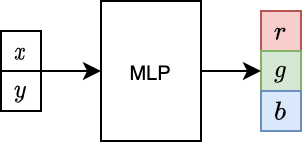
\includegraphics[width=0.3\textwidth]{images/inr}
    \end{figure}
    \item\pause We can generate the whole image by computing the value of $f_\varphi(x,y)$ at each coordinate
    \item\pause I.e. we have \textit{1 image} = \textit{1 INR}
\end{itemize}
\end{frame}


%\begin{frame}{Benefits of INRs}
%    \begin{itemize}
%        \item\pause They carry more ``complete'' information about a signal:
%        \begin{itemize}
%            \item Usual 2D arrays of pixels are discretized version of a signal
%            \item INRs are continuous and carry information ``between'' the pixels
%            \item This allows one to have ``superresolution out-of-the-box''
%        \end{itemize}
%        \item\pause They are popular in 3D deep learning since they are cheaper to generate and operate with than 3D objects
%        \begin{itemize}
%            \item\pause For 2D images the situation is not currently clear
%        \end{itemize}
%    \end{itemize}
%\end{frame}
%
%
%\begin{frame}{Problems with INRs}
%\begin{itemize}
%    \item\pause INRs are not that small:
%    \begin{itemize}
%        \item\pause SIREN/FFN use $\approx 256\times 5$ MLPs with 3000 epochs
%        \item\pause But fitting low-frequency images is much easier\footnote{a note to myself: show face/knot examples here}
%    \end{itemize}
%    \item\pause It requires to train an INR on an image to obtain the INR and each training procedure (currently) takes a lot of time (up to 10 minutes).
%    \item\pause Community does not have a good understanding of how to work with them
%\end{itemize}
%\end{frame}


%\begin{frame}{Transposed convolutions are problematic}
%\begin{itemize}
%    \item\pause They lack the biological plausibility of normal convolutions
%    \item\pause They produce artefacts (like checkerboard patterns)
%    \item\pause You have to change architecture for each output size
%    \begin{itemize}
%        \item\pause This can be solved by interpolation procedures to some extent, but for tasks like segmentation this would lead to coarse predictions
%    \end{itemize}
%    \item\pause They struggle to capture scene geometry:
%    \begin{itemize}
%        \item\pause For example, it's hard to draw long straight lines (so generated walls ``wobble'', circles are curved, etc)
%        \item\pause CoordConv paper showed that it cannot learn to classify a pixel given its coordinates
%    \end{itemize}
%\end{itemize}
%\end{frame}



\begin{frame}{INR-GAN}
\begin{itemize}
    \item\pause Main idea: train a generator to produce INRs
    \begin{figure}
        \centering
        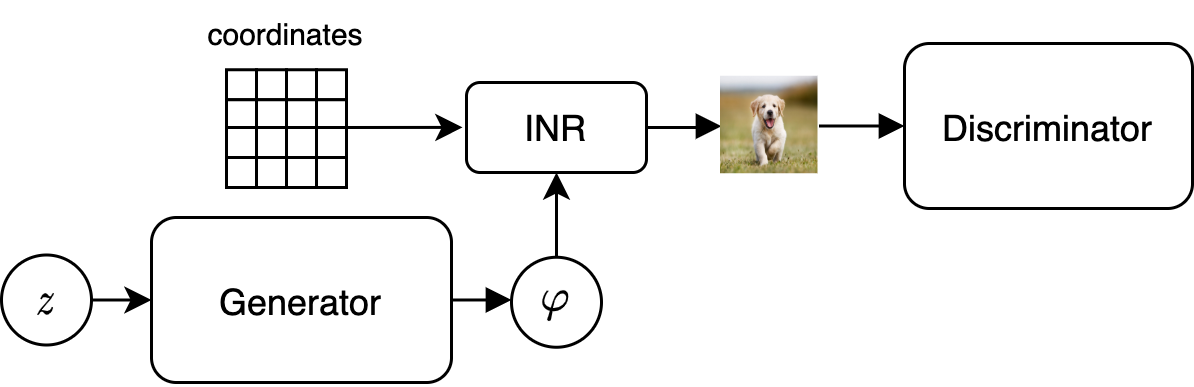
\includegraphics[width=0.9\textwidth]{images/inr-gan}
    \end{figure}
    \item\pause Discriminator can operate:
    \begin{itemize}
        \item\pause on top of images
        \item\pause on top of INRs (but this would require converting the whole dataset into INRs)
    \end{itemize}
\end{itemize}
\end{frame}


\begin{frame}{Advantages compared to traditional GANs}
\begin{itemize}
    \pause\item A unified generator architecture for images/audio/video/3D-shapes
    \pause\item Better biological plausibility
    \pause\item We can generate different resolutions for different parts of an image
    \begin{itemize}
        \pause\item Imagine that we generate an image of a human on a sky background
        \pause\item We can use dense set of coordinates for a human and a sparse set of coordinates for the sky
        \pause\item It is good since it is impossible to do so for a normal GAN
    \end{itemize}
    \pause\item We can generate spherical images (and images on any surface)
    \pause\item We can use ``random resolutions'' loss to train a high-resolution GAN
    \pause\item We can train our generator on images of extreme resolution by using a ``super-resolution'' loss:
    \begin{itemize}
        \pause\item Train an INR-GAN normally on, for example, $256\times256$ images
        \pause\item Additionally, compute random dense patches and make the discriminator to distinguish between real/fake dense patches
        \pause\item (Provide global context if needed)
    \end{itemize}
    \item\pause It should be cheaper to use for some domains (audio, 3D, video, extreme-resolution images)
    \item\pause Progressive growing is easier to incorporate
\end{itemize}
\end{frame}


\begin{frame}{Question: what other benefits can an INR-GAN have?}
What other benefits can an INR-GAN have compared to a traditional GAN?
\end{frame}


\begin{frame}{Current samples on LSUN bedroom 64x64}
\begin{figure}
    \centering
    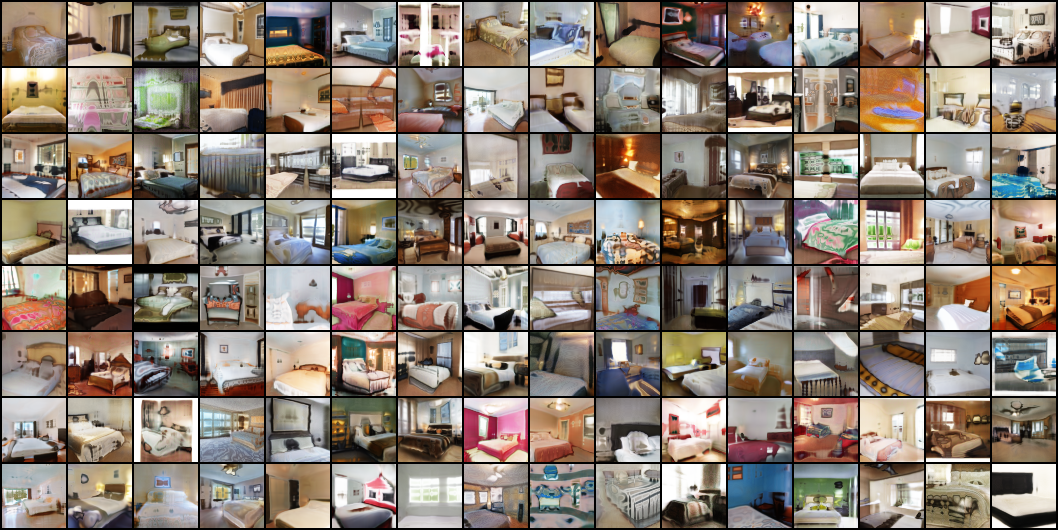
\includegraphics[width=\textwidth]{images/samples}
\end{figure}
\end{frame}


\begin{frame}{Interpolations on LSUN conference room 64x64}
\begin{figure}
    \centering
    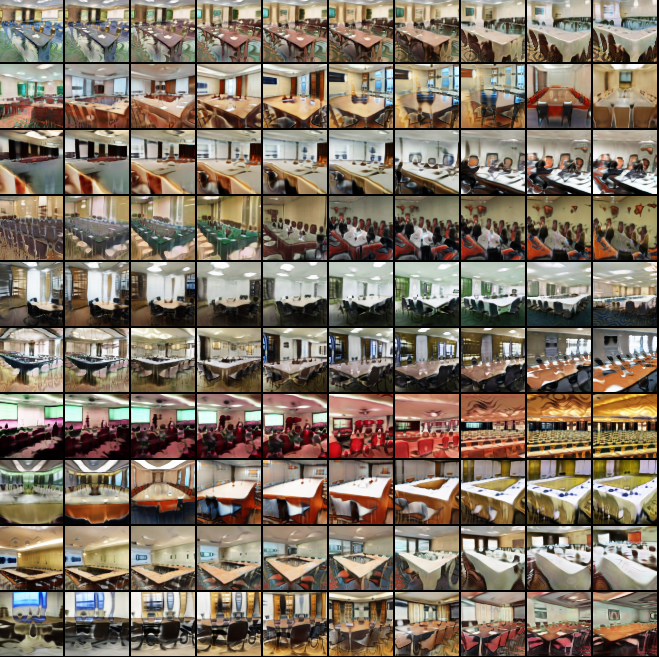
\includegraphics[width=0.7\textwidth]{images/interpolations-conference-room}
\end{figure}
\end{frame}

\begin{frame}{Interpolations on LSUN bedroom 64x64}
\begin{figure}
    \centering
    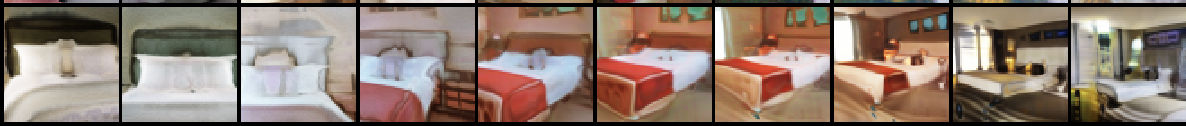
\includegraphics[width=0.7\textwidth]{images/interpolations-1}
\end{figure}
\begin{figure}
    \centering
    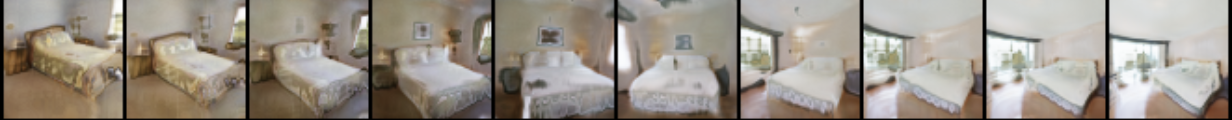
\includegraphics[width=0.7\textwidth]{images/interpolations-2}
\end{figure}
\begin{figure}
    \centering
    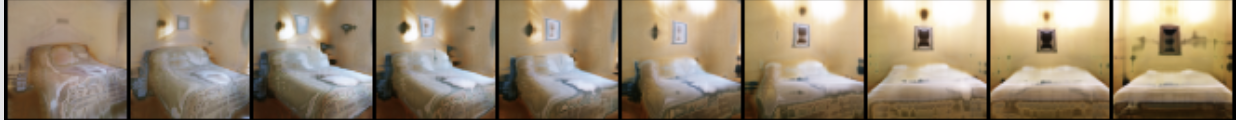
\includegraphics[width=0.7\textwidth]{images/interpolations-3}
\end{figure}
\begin{figure}
    \centering
    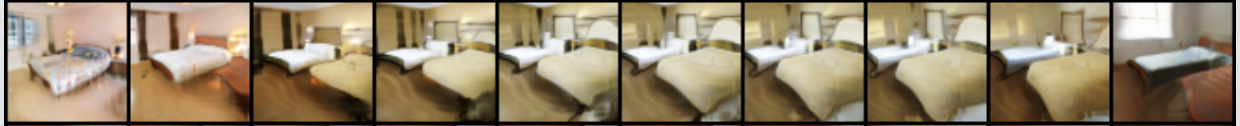
\includegraphics[width=0.7\textwidth]{images/interpolations-4}
\end{figure}
\begin{figure}
    \centering
    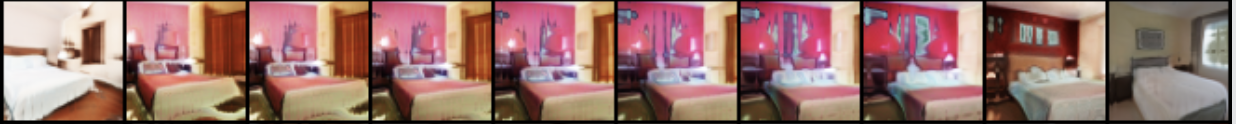
\includegraphics[width=0.7\textwidth]{images/interpolations-5}
\end{figure}
\begin{figure}
    \centering
    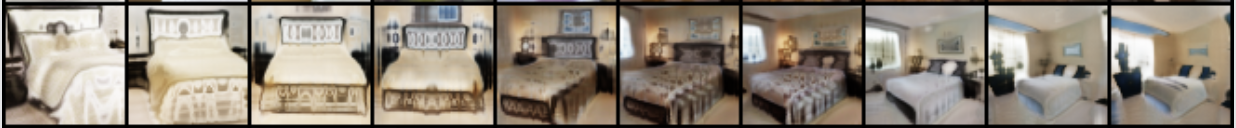
\includegraphics[width=0.7\textwidth]{images/interpolations-6}
\end{figure}
\end{frame}


\begin{frame}{Question 1: how to show ``geomtry understanding''}
    \begin{itemize}
        \item\pause CoordConv GAN paper claims that there interpolations are ``geometry-aware'': they are done through rotations, zooms, translations, etc.
        \item\pause In our experiments, we have found the same property
        \item\pause We have not checked if it is true for StyleGAN (it is likely to be true)
        \item\pause If it is true for StyleGAN, it does not mean that it was \textit{more difficult} for it to learn this geometry information (i.e. it could spend a lot of capacity on it).
        \item\pause How can we demonstrate that our model captures the geometry more easily?
    \end{itemize}
\end{frame}


\begin{frame}{Question 2: stability}
\begin{figure}
\centering
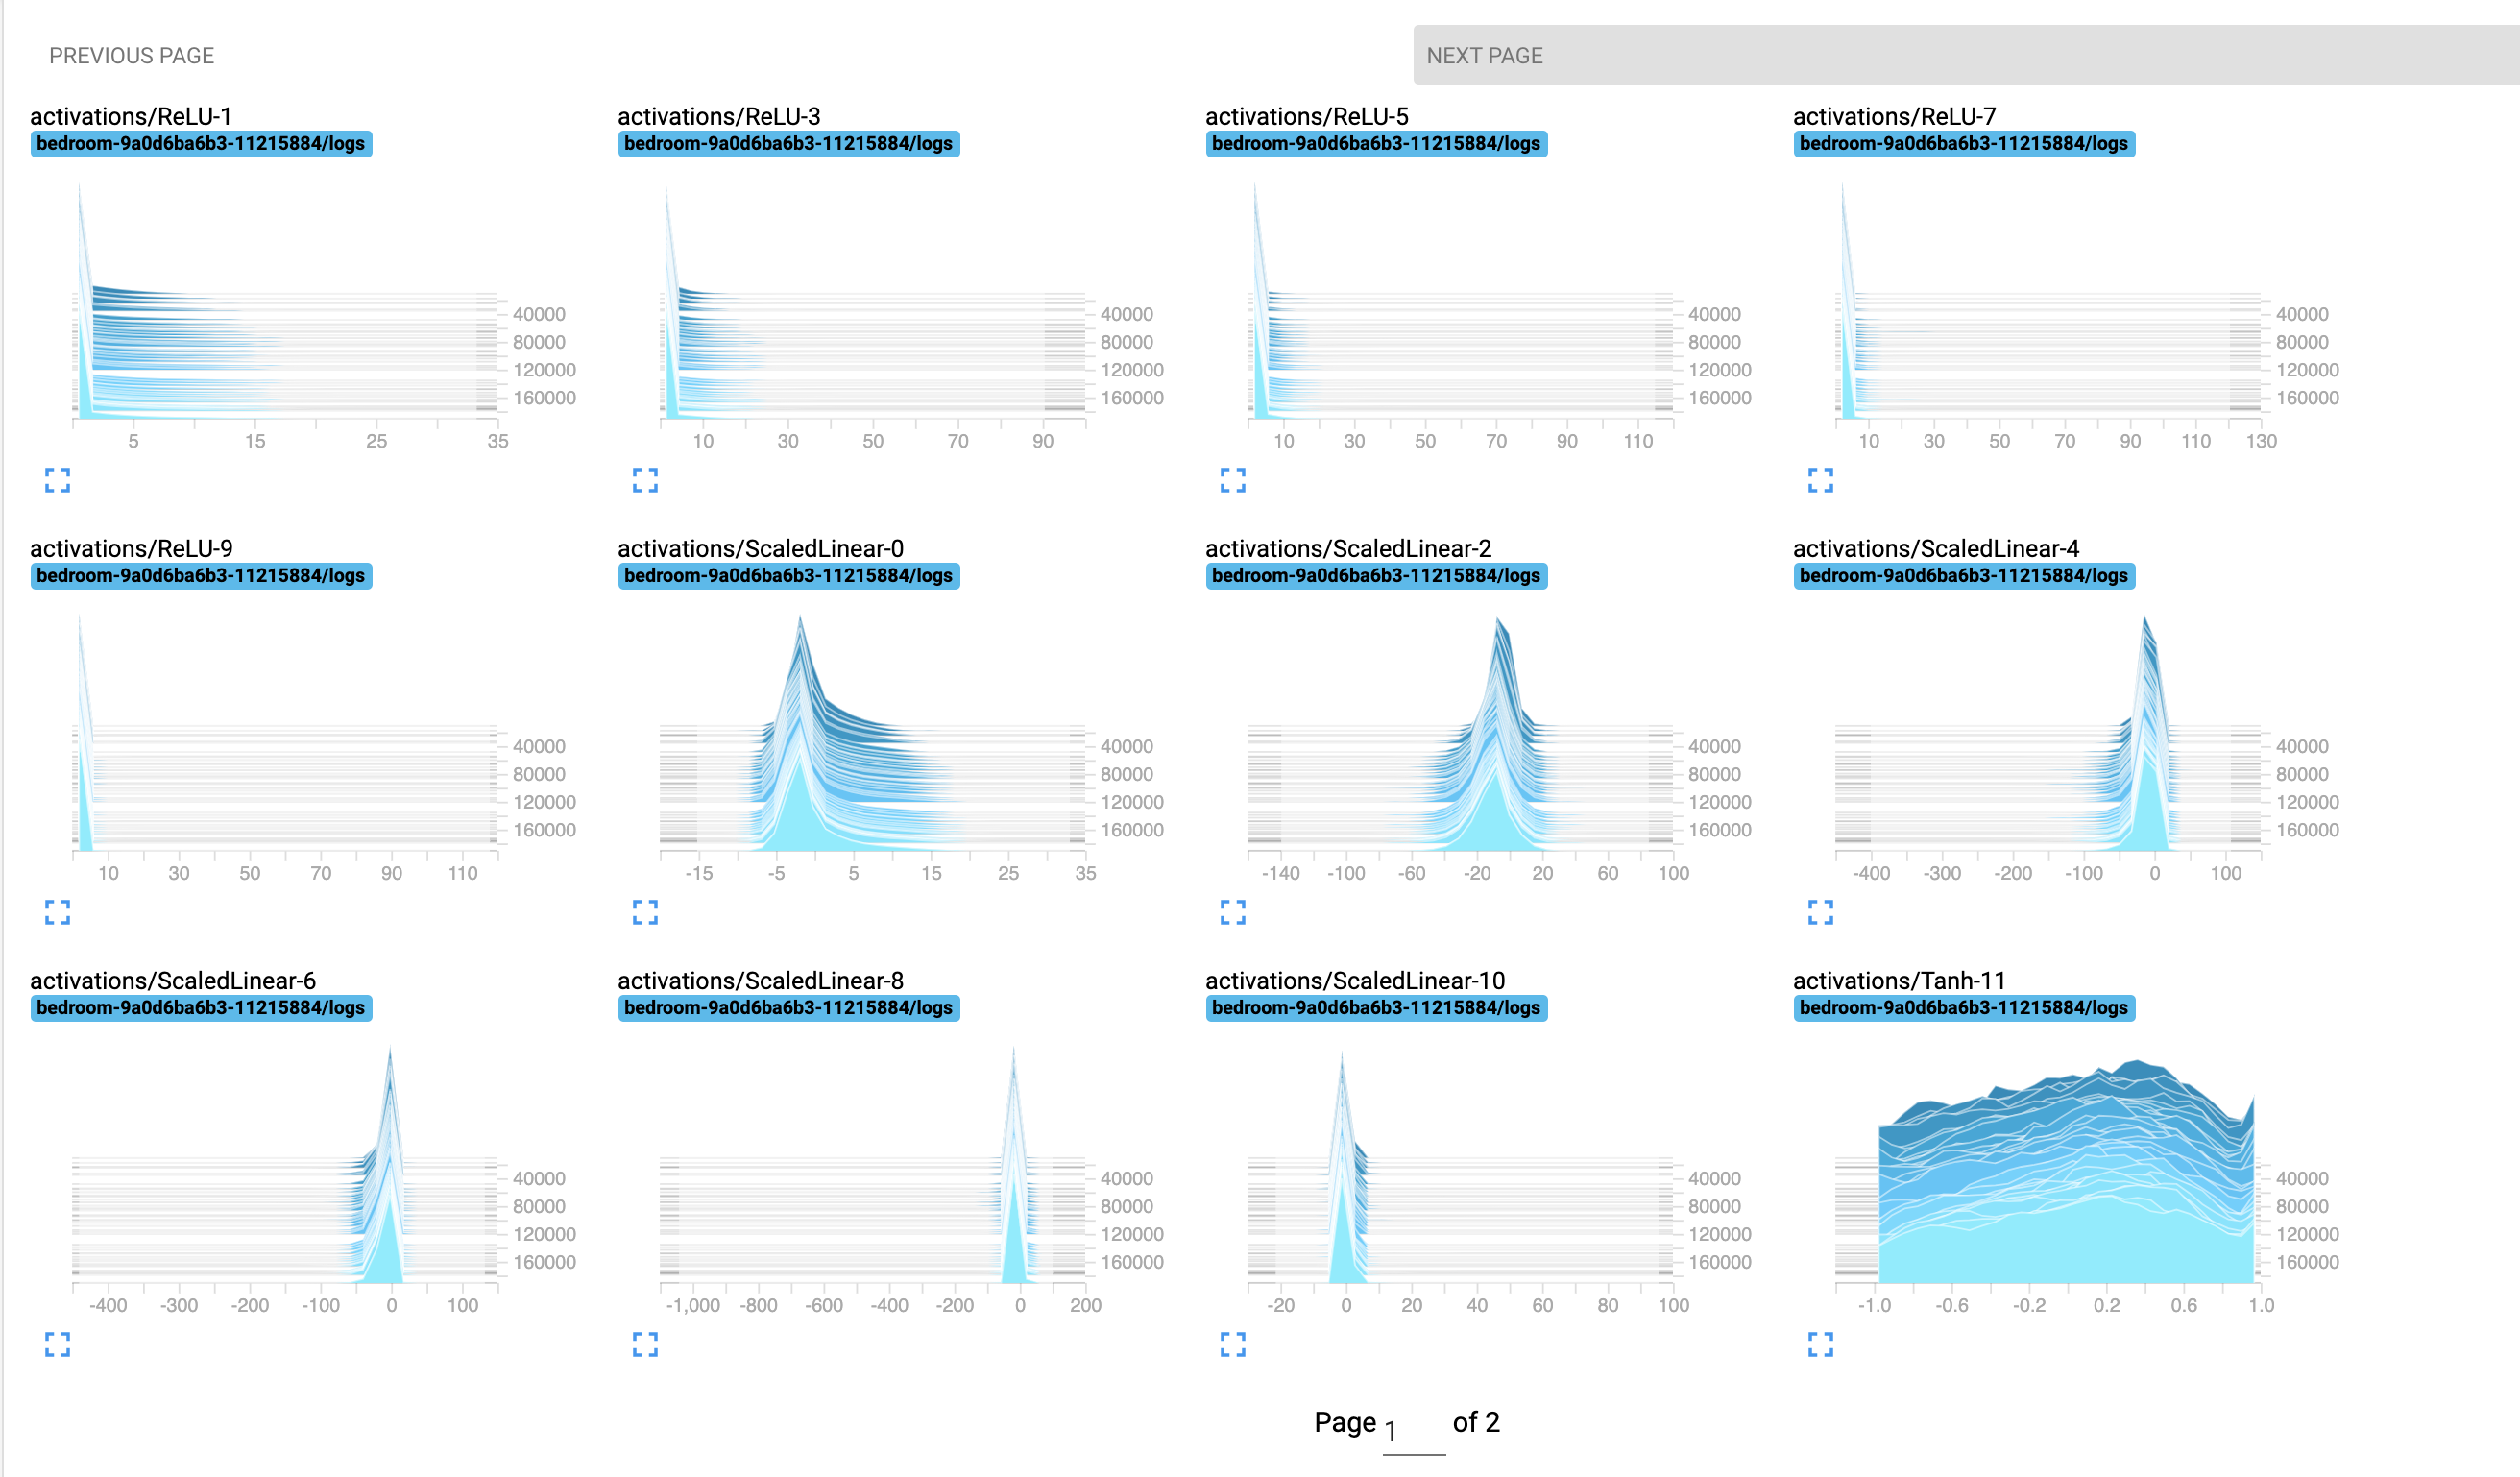
\includegraphics[width=\textwidth]{images/activations-hists}
\end{figure}
\begin{itemize}
    \item\pause Do we have a stability problem? How to alleviate it?
    \item\pause It's important to solve it since it's important to learn with a high LR 
\end{itemize}
\end{frame}




\begin{frame}{Question: abrupt interpolations problem}
\pause
Sometimes during interpolations we have a very abrupt change

\pause
\begin{figure}
    \centering
    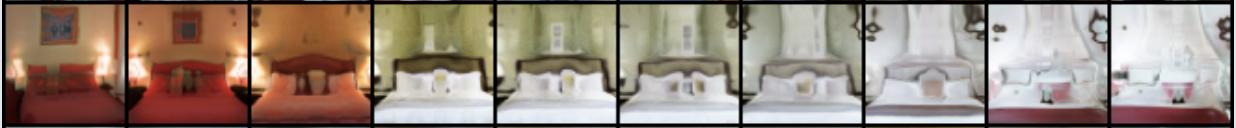
\includegraphics[width=0.7\textwidth]{images/abrupt-changes-1}
\end{figure}
\begin{figure}
    \centering
    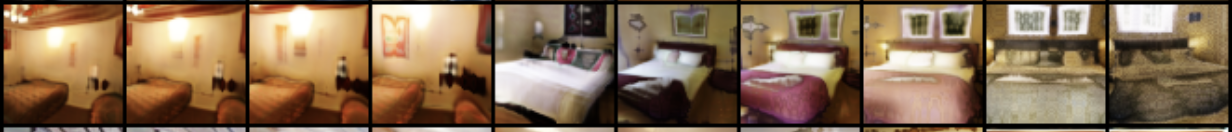
\includegraphics[width=0.7\textwidth]{images/abrupt-changes-2}
\end{figure}

\pause
What can be the cause of it and how to alleviate it?
\end{frame}

\end{document}
